
\de{ĐỀ THI HỌC KỲ I NĂM HỌC 2022-2023}{Trường THPT Nguyễn Văn Cừ - Quảng Nam}
\begin{center}
	\textbf{PHẦN 1 - TRẮC NGHIỆM}
\end{center}
\Opensolutionfile{ans}[ans/ans]
%%==========Câu 1
\begin{ex}%[0D2Y2-1]%[Dự án đề kiểm tra HKI NH22-23- Nguyễn Văn Sơn]%[THPT Nguyễn Văn Cừ - Quảng Nam]
	Hệ nào dưới đây là hệ bất phương trình bậc nhất hai ẩn?
	\choice
	{$\heva{&x+2y^3>0\\ & x\leq 0}$}
	{\True $\heva{&x-2y>0\\ & x\leq 0}$}
	{$\heva{&x-2y>0\\ & x^2-y\leq 0}$}
	{$\heva{&x-y>0\\ & x+4y^2\leq 0}$}
	\loigiai{
		Hệ $\heva{&x-2y>0\\ & x\leq 0}$ là hệ bất phương trình bậc nhất hai ẩn.
	}
\end{ex}
%%==========Câu 2
\begin{ex}%[0D1Y2-1]%[Dự án đề kiểm tra HKI NH22-23- Nguyễn Văn Sơn]%[THPT Nguyễn Văn Cừ - Quảng Nam]
	Cho tập hợp $A=\left\{n \in \mathbb{N} \mid n \leq 5\right\}$. Tập hợp \(A\) viết dưới dạng liệt kê các phần tử là
	\choice
	{$A=\left\{1 ; 2 ; 3 ; 4 ; 5 ; 6\right\}$}
	{\True $A=\left\{0 ; 1 ; 2 ; 3 ; 4 ; 5\right\}$}
	{ $A=\left\{1 ; 2 ; 3 ; 4 ; 5\right\}$}
	{$A=\left\{0 ; 1 ; 2 ; 3 ; 4 ; 5 ; 6\right\}$}
	\loigiai{
		Ta có $n \in \mathbb{N}$ và $n \leq 5$ nên $0\leq n \leq 5$.
		Vậy $A=\left\{0 ; 1 ; 2 ; 3 ; 4 ; 5\right\}$.
	}
\end{ex}

%%==========Câu3
\begin{ex}%[0X1B1-3]%[Dự án đề kiểm tra HKI NH22-23- Nguyễn Văn Sơn]%[THPT Nguyễn Văn Cừ - Quảng Nam]
	Số quy tròn của số gần đúng $673582$ với độ chính xác $d=500$ là
	\choice
	{\True $674000$}
	{$673000$}
	{$673600$}
	{$673500 $}
	\loigiai{
		Vì độ chính xác đến hàng trăm nên ta quy tròn đến hàng nghìn do đó
		số quy tròn của số gần đúng $673582$ với độ chính xác $d=500$ là $674000$.
	}
\end{ex}

%%==========Câu 4
\begin{ex}%[0H1Y1-1]%[Dự án đề kiểm tra HKI NH22-23- Nguyễn Văn Sơn]%[THPT Nguyễn Văn Cừ - Quảng Nam]
	Cho góc lượng giác $\alpha$ thoả mãn $90^{\circ}<\alpha<180^{\circ}$. Mệnh đề nào dưới đây \textbf{đúng}?
	\choice
	{$\cos \alpha>0$}
	{$\cot \alpha>0$}
	{$\tan \alpha>0$}
	{\True $\sin \alpha>0$}
	\loigiai{
		Do $\alpha$ là góc tù nên $\sin \alpha>0$.
	}
\end{ex}
%%==========Câu 5
\begin{ex}%[0D1Y1-1]%[Dự án đề kiểm tra HKI NH22-23- Nguyễn Văn Sơn]%[THPT Nguyễn Văn Cừ - Quảng Nam]
	Phát biểu nào dưới đây \textbf{\textit{là một mệnh đề}}?
	\choice
	{$x<3$}
	{Bạn có đi chơi không?}
	{\True Hà Nội là thủ đô của Việt Nam}
	{Mùa thu Hà Nội thật đẹp!}
	\loigiai{
		"Hà Nội là thủ đô của Việt Nam" là một mệnh đề.	
	}
\end{ex}
%%==========Câu 6
\begin{ex}%[0H2B1-2]%[Dự án đề kiểm tra HKI NH22-23- Nguyễn Văn Sơn]%[THPT Nguyễn Văn Cừ - Quảng Nam]
	Gọi $M$, $N$ lần lượt là trung điểm của các cạnh $AB, AC$ của tam giác đều $ABC$. Hỏi cặp vec-tơ nào sau đây cùng hướng?
	\choice
	{\True $\Vec{AB}$ và $\vec{MB}$}
	{$\Vec{MN}$ và $\vec{CB}$}
	{$\Vec{MA}$ và $\vec{MB}$}
	{$\Vec{AN}$ và $\vec{CA}$}
	\loigiai{
		\begin{center}
			\begin{tikzpicture}[line join=round, line cap=round,>=stealth,thick]
			\coordinate[label=above:$A$] (A) at (2,3);
			\coordinate[label=below left:$B$] (B) at (0,0);
			\coordinate[label=below right:$C$] (C) at (4,0);
			\coordinate[label=left:$M$] (M) at ($(A)!.5!(B)$);
			\coordinate[label=right:$N$] (N) at ($(A)!.5!(C)$);
			\draw(A)--(B)--(C)--(A)--(M)--(N);
		\end{tikzpicture}
		\end{center}
		Dựa vào hình vẽ ta có $\Vec{AB}$ và $\vec{MB}$ cùng hướng với nhau.
	}
\end{ex}
%%==========Câu 7
\begin{ex}%[0H2Y2-3]%[Dự án đề kiểm tra HKI NH22-23- Nguyễn Văn Sơn]%[THPT Nguyễn Văn Cừ - Quảng Nam]
	Cho ba điểm $A,B,C$ phân biệt. Khẳng định nào sau đây \textbf{đúng}?
	\choice
	{\True $\Vec{AC}+\vec{CB}=\vec{AB}$}
	{$\Vec{AB}+\vec{BC}=\vec{CA}$}
	{$\Vec{BA}-\vec{BC}=\vec{AC}$}
	{$\Vec{CA}+\vec{CB}=\vec{AB}$}
	\loigiai{Áp dụng quy tắc 3 điểm ta có $\Vec{AC}+\vec{CB}=\vec{AB}$.
	}
\end{ex}	
%%==========Câu 8
\begin{ex}%[0H3Y1-3]%[Dự án đề kiểm tra HKI NH22-23- Nguyễn Văn Sơn]%[THPT Nguyễn Văn Cừ - Quảng Nam]
	Trong hệ toạ độ $Oxy$, cho $A(5;2), B(10;8)$. Tìm toạ độ của vec-tơ $\vec{AB}$.
	\choice
	{\True$\vec{AB}=(5;6)$}
	{$\Vec{AB}=(2;4)$}
	{$\Vec{AB}=(15;10)$}
	{$\Vec{AB}=(50;16)$}
	\loigiai{ Ta có $\vec{AB}=(x_B-x_A;y_B-y_A)$ nên $\vec{AB}=(10-5;8-2)=(5;6)$.
		
	}
\end{ex}
%%==========Câu 9
\begin{ex}%[0H3Y2-1]%[Dự án đề kiểm tra HKI NH22-23- Nguyễn Văn Sơn]%[THPT Nguyễn Văn Cừ - Quảng Nam]
	Cho hai vec-tơ $\vec{a}$ và $\vec{b}$ khác $\vec{0}$, $\alpha$ là góc giữa hai vec-tơ $\vec{a}$ và $\vec{b}$. Tích vô hướng $\vec{a}\cdot\vec{b}$ là 
	\choice
	{$\vec{a}\cdot\vec{b}=-|\vec{a}|\cdot|\vec{b}|$}
	{$\vec{a}\cdot\vec{b}=|\vec{a}|\cdot|\vec{b}|\sin\alpha$}
	{$\vec{a}\cdot\vec{b}=|\vec{a}|\cdot|\vec{b}|$}
	{\True $\vec{a}\cdot\vec{b}=|\vec{a}|\cdot|\vec{b}|\cos\alpha$}
	\loigiai{Theo định nghĩa tích vô hướng của hai vec-tơ ta có $\vec{a}\cdot\vec{b}=|\vec{a}|\cdot|\vec{b}|\cos\alpha$}.
\end{ex}
%%==========Câu 10
\begin{ex}%[0H2Y1-4]%[Dự án đề kiểm tra HKI NH22-23- Nguyễn Văn Sơn]%[THPT Nguyễn Văn Cừ - Quảng Nam]
	Cho hai điểm $A$ và $B$ phân biệt. Điều kiện để $I$ là trung điểm $AB$ là
	\choice
	{$IA=2\cdot IB$}
	{\True$\vec{IA}=-\vec{IB}$}
	{$\vec{IA}=\vec{IB}$}
	{$\vec{AI}=\vec{BI}$}
	\loigiai{Theo giả thiết $I$ là trung điểm của $AB$ khi $IA=IB$ và hai vec-tơ ta có $\vec{IA}, \vec{IB}$ ngược chiều hay $\vec{IA}=-\vec{IB}$.
		
	}
\end{ex}	
%%==========Câu 11
\begin{ex}%[0H1Y1-1]%[Dự án đề kiểm tra HKI NH22-23- Nguyễn Văn Sơn]%[THPT Nguyễn Văn Cừ - Quảng Nam]
	Cho góc $\alpha$ thỏa mãn $0^\circ \leq \alpha \leq 180^\circ$. Khẳng định nào sau đây \textbf{đúng}?
	\choice
	{$\cos\left(180^\circ - \alpha \right)=\cos\alpha$}
	{$\tan\left(180^\circ - \alpha \right)=\tan\alpha$}
	{\True $\sin\left(180^\circ - \alpha \right)=\sin\alpha$}
	{$\cot\left(180^\circ - \alpha \right)=\cot\alpha$}
	\loigiai
	{
		Hai góc bù nhau thì $\sin$ sẽ bằng nhau nên $\sin\left(180^\circ - \alpha \right)=\sin\alpha$.
	}
\end{ex}
%%==========Câu 12
\begin{ex}%[0H2Y1-3]%[Dự án đề kiểm tra HKI NH22-23- Nguyễn Văn Sơn]%[THPT Nguyễn Văn Cừ - Quảng Nam]
	Cho hình bình hành $ABCD$ (\textit{như hình vẽ sau}). Đẳng thức nào sau đây \textbf{đúng}?
	\choice
	{\True $\overrightarrow{AD}=\overrightarrow{BC}$}
	{$\overrightarrow{AB}=\overrightarrow{CD}$}
	{$\overrightarrow{BC}=\overrightarrow{DA}$}
	{$\overrightarrow{AC}=\overrightarrow{BD}$}
	\loigiai
	{
		\begin{center}
			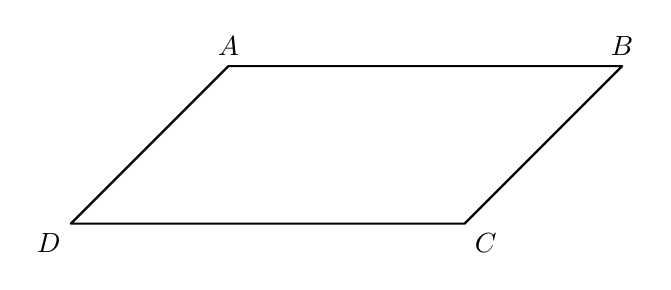
\begin{tikzpicture}[line join=round, line cap=round,>=stealth,thick]
				\coordinate[label=above:$A$] (A) at (2,2);
				\coordinate[label=above:$B$] (B) at (7,2);
				\coordinate[label=below right:$C$] (C) at (5,0);
				\coordinate[label=below left:$D$] (D) at (0,0);
				\draw(A)--(B)--(C)--(D)--(A);
			\end{tikzpicture}
		\end{center}
	Do $\overrightarrow{AD}$ và $\overrightarrow{BC}$ cùng hướng và có độ dài bằng nhau nên $\overrightarrow{AD}=\overrightarrow{BC}$.
	}
\end{ex}
%%==========Câu 13
\begin{ex}%[0H1Y2-2]%[Dự án đề kiểm tra HKI NH22-23- Nguyễn Văn Sơn]%[THPT Nguyễn Văn Cừ - Quảng Nam]
	Cho tam giác $ABC$ có độ dài ba cạnh là $BC=a, AC=b, AB=c$. Gọi $R$ là bán kính đường tròn ngoại tiếp và $S$ là diện tích tam giác $ABC$. Mệnh đề nào dưới đây \textbf{đúng}?
	\choice
	{$S=\dfrac{ac}{4R}$}
	{\True $S=\dfrac{abc}{4R}$}
	{$S=\dfrac{abc}{R}$}
	{$S=\dfrac{R}{4abc}$}
	\loigiai
	{
		Theo công thức tính diện tích tam giác ta có $S=\dfrac{abc}{4R}$.
	}
\end{ex}
%%==========Câu 14
\begin{ex}%[0D2Y1-1]%[Dự án đề kiểm tra HKI NH22-23- Nguyễn Văn Sơn]%[THPT Nguyễn Văn Cừ - Quảng Nam]
	Cặp số $(1;-1)$ \textbf{\textit{thuộc miền nghiệm}} của bất phương trình nào sau đây?
	\choice
	{$-x-y<0$}
	{\True $x+3y+1<0$}
	{$x+y-3>0$}
	{$-x-3y-1<0$}
	\loigiai
	{
		Thế cặp số $(1;-1)$ lần lượt vào từng phương án ta chỉ thấy khi thế vào bất phương trình $x+3y+1<0$ là thỏa mãn vì $1+3(-1)+1=-1<0$.
	}
\end{ex}
%%==========Câu 15
\begin{ex}%[0H2B4-1]%[Dự án đề kiểm tra HKI NH22-23- Nguyễn Văn Sơn]%[THPT Nguyễn Văn Cừ - Quảng Nam]
	Cho tam giác $ABC$ vuông tại $A$ và có $\widehat{ABC}=40^\circ$. Tính $\left(\overrightarrow{CA},\overrightarrow{CB}\right)$ (góc giữa hai vec-tơ $\overrightarrow{CA}$ và $\overrightarrow{CB}$ ).
	\choice
	{$\left(\overrightarrow{CA},\overrightarrow{CB}\right)=40^\circ$}
	{\True $\left(\overrightarrow{CA},\overrightarrow{CB}\right)=50^\circ$}
	{$\left(\overrightarrow{CA},\overrightarrow{CB}\right)=130^\circ$}
	{$\left(\overrightarrow{CA},\overrightarrow{CB}\right)=140^\circ$}
	\loigiai
	{
	
		\begin{center}
		\begin{tikzpicture}[line join=round, line cap=round,>=stealth,thick]
			\coordinate[label=left:$A$] (A) at (0,0);
			\coordinate[label=right:$B$] (B) at (6,0);
			\coordinate[label=above:$C$] (C) at (0,3);
			\draw(A)--(B)--(C)--(A);
			\draw pic[draw=black, angle eccentricity=0.75, angle radius=0.2cm]{right angle=C--A--B};
			\draw pic[" $ 40^\circ $ ", draw=black, angle eccentricity=1.5, angle radius=1.0cm]
			{angle=C--B--A}; 
		\end{tikzpicture}
		\end{center}
	Ta có $\left(\overrightarrow{CA},\overrightarrow{CB}\right)=\widehat{ACB}=90^\circ - \widehat{ABC}=90^\circ - 40^\circ = 50^\circ$.
	}
\end{ex}

\Closesolutionfile{ans}
%\begin{center}
%	\textbf{ĐÁP ÁN}
%	\inputansbox{10}{ans/ans}	
%\end{center}
\begin{center}
	\textbf{PHẦN 2 - TỰ LUẬN}
\end{center}

\begin{bt}%[0D1Y3-1]%[Dự án đề kiểm tra HK Toán 10-TinDatTran]%[THPT Nguyễn Văn Cừ - Quảng Nam]
Cho tập hợp $A=\{2 ; 3 ; 5 ; 7\}$ và $B=\{1 ; 2 ; 3 ; 4\}$. Hãy tìm các tập $A \cap B$, $A \cup B$, $A \setminus B$, $B \setminus A$.
\loigiai{
Ta có
\begin{itemize}
\item $A\cap B=\left\{2;3\right\}$;
\item $A\cup B=\left\{1;2;3;4;5;7\right\}$;
\item $A\setminus B=\left\{5;7\right\}$;
\item $B\setminus A=\left\{1;4\right\}$.
\end{itemize}
}
\end{bt}
\begin{bt}%[0H1B3-2]%[Dự án đề kiểm tra HK Toán 10-TinDatTran]%[THPT Nguyễn Văn Cừ - Quảng Nam]
\immini{Từ vị trí $A$ người ta quan sát một cây cao, giả sử $BC$ là chiều cao của cây (như hình vẽ). Người ta đo được khoảng cách $AB=15$m, góc $\widehat{CAB}=60^\circ$ và $\widehat{ABC}=73^\circ$. Tính chiều cao $BC$ của cây (kết quả làm tròn đến 2 chữ thập phân).}
{
\tikzset{
	ex_markstyle/.style={},
	ex_mark/.style  n args={1}{decoration={ markings, %
			mark= at position 0.5 with
			with{
				\ifnum#1=1
				\draw[ex_markstyle] (0pt,-2pt) -- (0pt,2pt);
				\fi
				\ifnum#1=2
				\draw[ex_markstyle] (-1pt,-2pt) -- (-1pt,2pt);
				\draw[ex_markstyle] (1pt,-2pt) -- (1pt,2pt);
				\fi
				\ifnum#1=3
				\draw[ex_markstyle] (-2pt,-2pt) -- (-2pt,2pt);
				\draw[ex_markstyle] (0pt,-2pt) -- (0pt,2pt);
				\draw[ex_markstyle] (2pt,-2pt) -- (2pt,2pt);
				\fi
				\ifnum#1=4
				\draw[ex_markstyle] (-1pt,-1pt) -- (1pt,1pt);
				\draw[ex_markstyle] (-1pt,1pt) -- (1pt,-1pt);
				\fi
		}},
		pic actions/.append code=\tikzset{postaction=decorate}},
}
%------
\definecolor{lightcornflowerblue}{rgb}{0.6, 0.81, 0.93}
\definecolor{cadmiumgreen}{rgb}{0.0, 0.42, 0.24}
\definecolor{trueblue}{rgb}{0.0, 0.45, 0.81}
\definecolor{tumbleweed}{rgb}{0.87, 0.67, 0.53}%màu cát
\definecolor{forestgreen(web)}{rgb}{0.13, 0.55, 0.13}
\definecolor{darkpastelgreen}{rgb}{0.01, 0.75, 0.24}
\definecolor{bronze}{rgb}{0.8, 0.5, 0.2}
\begin{tikzpicture}[line join=round, line cap=round,scale=1.5,transform shape]
	\tikzset{cay/.pic={
			\def\T{ %Thân
				(-.33,0)%trái
				..controls +(-50:.25) and +(40:.45) ..  (-.57,-1.45)
				..controls +(20:.1) and +(-160:.15) ..  (-.1,-1.3)
				..controls +(-120:.1) and +(60:.15) ..  (-.2,-1.6)
				..controls +(-30:.1) and +(-140:.15) ..  (.15,-1.3)
				..controls +(-20:.1) and +(-160:.15) ..  (.57,-1.4)
				..controls +(170:.4) and +(-160:.1) ..  (.35,0)
				..controls +(110:.5) and +(80:.5) ..  (-.33,0)
				;}
			%\draw \T;
			\fill[bronze] \T;
			\def\C{ 
				(0,.3)
				..controls +(-100:.25) and +(-60:.2) ..  (-.3,.1)
				..controls +(-100:.25) and +(-60:.2) ..  (-.6,0)
				..controls +(-120:.45) and +(-110:.35) ..  (-1,.2)
				..controls +(-150:.5) and +(-140:.35) ..  (-1.15,.7)%nút giao
				..controls +(-170:.4) and +(-170:.35) ..  (-1,1.15)
				..controls +(140:.35) and +(110:.4) ..  (-.37,1.35)
				..controls +(110:.25) and +(80:.3) ..  (-.15,1.35)
				..controls +(80:.3) and +(95:.8) ..  (.55,1.1)
				..controls +(80:.2) and +(95:.2) ..  (.8,1.1)
				..controls +(20:.1) and +(95:.1) ..  (.95,1)
				..controls +(-20:.4) and +(35:.25) ..  (1,.47)
				..controls +(-30:.3) and +(-20:.3) ..  (.75,0.05)%nút giao
				..controls +(-120:.3) and +(-60:.2) ..  (.35,0)
				..controls +(175:.2) and +(-160:.1) ..  (.2,0.2)
				..controls +(-160:.1) and +(-70:.1) ..  (0,.3)
				;}
			\draw \C;
			\fill[forestgreen(web)] \C;
			\def\C1{ 
				(-1.15,.7)%nút giao
				..controls +(-170:.4) and +(-170:.35) ..  (-1,1.15)
				..controls +(140:.35) and +(110:.4) ..  (-.37,1.35)
				..controls +(110:.25) and +(80:.3) ..  (-.15,1.35)
				..controls +(80:.3) and +(95:.8) ..  (.55,1.1)
				..controls +(80:.2) and +(95:.2) ..  (.8,1.1)
				..controls +(20:.1) and +(95:.1) ..  (.95,1)
				..controls +(-20:.4) and +(35:.25) ..  (1,.47)
				..controls +(-50:.5) and +(-85:.6) ..  (.65,.55)% gần nút giao
				..controls +(-160:.4) and +(-120:.4) ..  (0,.7)
				..controls +(-150:.2) and +(-80:.4) ..  (-.63,.6)
				..controls +(-140:.5) and +(-130:.4) ..  (-1.15,.7)
				;}
			%\draw \C1;
			\fill[darkpastelgreen] \C1;
			\def\G{ %Gân
				(-.8,.2)
				..controls +(-35:.1) and +(130:.35) ..  
				(-.32,0)%nút giao
				..controls +(-40:.1) and +(45:.35) ..  (-.42,-1.25)
				(-.32,0)%nút giao
				..controls +(120:.1) and +(-45:.35) ..  (-.58,.45)
				(-.32,0)%nút giao
				..controls +(80:.1) and +(-170:.35) ..  (-.05,.45)
				(-.28,.3)
				..controls +(80:.1) and +(-60:.05) ..  (-.35,.55)
				%Gân phải
				(.45,-1.3)
				..controls +(130:.6) and +(-160:.3) ..  (.6,0.35)
				(.37,0)
				..controls +(35:.2) and +(-150:.1) ..  (.66,0.15)
				(.37,0)
				..controls +(80:.2) and +(-40:.1) ..  (.18,0.4)
				(.31,0.25)
				..controls +(80:.1) and +(-150:.1) ..  (.38,0.5)
				(.25,-0.15)
				..controls +(-110:.05) and +(110:.05) ..  (.2,-0.5)%gân dọc
				(.2,-0.25)
				..controls +(-110:.05) and +(110:.05) ..  (.17,-0.45)
				(-.2,-0.15)
				..controls +(-70:.1) and +(110:.05) ..  (-.18,-0.5)
				(-.15,-0.15)
				..controls +(-70:.1) and +(110:.05) ..  (-.15,-0.7)
				(-.05,-0.8)
				..controls +(-80:.15) and +(-10:.15) ..  (-.3,-1.28)
				(-.1,-0.9)
				..controls +(-110:.1) and +(20:.05) ..  (-.2,-1.1)
				(.1,-1)
				..controls +(-50:.05) and +(120:.05) ..  (.15,-1.2)
				(.1,-1.15)
				..controls +(-50:.05) and +(120:.05) ..  (.12,-1.2)
				(.15,-.75)
				..controls +(-120:.1) and +(-140:.1) ..  (.22,-.9)
				..controls +(70:.12) and +(120:.05) ..  (.18,-.9)
				;}
			
			\draw \G;
			
	}}
	\path
	(2,0)pic[scale=.8]{cay}
	;
	\path 	(2,-1.1) coordinate (B)
	(2,1.25) coordinate (C)
	($(B)!1!73:(C)$) coordinate (Bt)
	($(C)!1!-47:(B)$) coordinate (Ct)
	(intersection of B--Bt and C--Ct) coordinate (A)
	;
	\node at (B) [below]{\tiny $B$};
	\node at (A) [left]{\tiny $A$};
	\node at (C) [above]{\tiny $C$};
	\draw (A)--(B)--(C)--cycle;
	\draw    pic["\tiny $60^\circ$", draw=black, angle eccentricity=1.5,angle radius=.4cm]
	{angle=B--A--C}; 
	\draw pic["\tiny $73^\circ$", draw=black,double, angle eccentricity=1.3,angle radius=.4cm]
	{angle=C--B--A};
\end{tikzpicture}
}
\loigiai{
Tam giác $ABC$ có $C=180^\circ-(A+B)=180^\circ-(60^\circ+73^\circ)=47^\circ$.\\
Theo định lý Sin ta có 
\[\dfrac{BC}{\sin A}=\dfrac{AB}{\sin C}\Rightarrow BC=\dfrac{AB}{\sin C}\cdot BC=\dfrac{15}{\sin 47^\circ}\cdot \sin 60^\circ\approx17{,}76~(\mathrm{m}).\]
}
\end{bt}
\begin{bt}%[0H3B1-3]%[0H2B2-1]%[Dự án đề kiểm tra HK Toán 10-TinDatTran]%[THPT Nguyễn Văn Cừ - Quảng Nam]
\begin{enumerate}
\item Trong mặt phẳng toạ độ $Oxy$ cho ba điểm $A(1;-5)$, $B(2;3)$ và $C(-2;4)$. Tìm toạ độ điểm $M$ sao cho $\overrightarrow{AM}=\overrightarrow{AB}+3 \cdot \overrightarrow{BC}$.
\item Cho bốn điểm bất kỳ $A , B, C, D$. Chứng minh rằng:
\[\overrightarrow{AC}+\overrightarrow{BD}+\overrightarrow{CB}+\overrightarrow{DA}=\overrightarrow{0}.\]
\end{enumerate}
\loigiai{
\begin{enumerate}
\item Gọi $M(x;y)$ là điểm cần tìm. Ta có $\overrightarrow{AB}=(1;8)$; $\overrightarrow{BC}=(-4;1)$;  $\overrightarrow{AM}=(x-1;y+5)$.\\
Ta có 
\[\overrightarrow{AM}=\overrightarrow{AB}+3 \cdot \overrightarrow{BC}\Leftrightarrow \heva{&x-1=1+3\cdot (-4)\\&y+5=8+3\cdot 1}\Leftrightarrow\heva{&x=-10\\&y=6.}\]
Vậy $M(-10;6)$ là điểm cần tìm.
\item 
Ta có
\begin{eqnarray*}
\allowdisplaybreaks
\overrightarrow{AC}+\overrightarrow{BD}+\overrightarrow{CB}+\overrightarrow{DA}=\left(\overrightarrow{DA}+\overrightarrow{AC}\right)+\left(\overrightarrow{CB}+\overrightarrow{BD}\right)=\overrightarrow{DC}+\overrightarrow{CD}=\overrightarrow{DD}=\overrightarrow{0}.
\end{eqnarray*}
\end{enumerate}
}
\end{bt}
\begin{bt}%[0H2K4-1]%[Dự án đề kiểm tra HK Toán 10-TinDatTran]%[THPT Nguyễn Văn Cừ - Quảng Nam]
Cho hình vuông $ABCD$, điểm $M$ nằm trên đoạn $BD$ sao cho $B M=\dfrac{1}{4} BD$, điểm $N$ là trung điểm của đoạn thẳng $AD$. Tính tích vô hướng $\overrightarrow{MC} \cdot \overrightarrow{MN}$.
\loigiai{
\begin{center}
\begin{tikzpicture}
	\path
	(0,3) coordinate (A)
	(3,3) coordinate (B)
	(3,0) coordinate (C)
	(0,0) coordinate (D)
	($(B)!1/4!(D)$) coordinate (M)
	($(A)!.5!(D)$) coordinate (N)
	;
	\draw (A)--(B)--(C)--(D)--cycle (M)--(C) (M)--(N) (B)--(D);
	\foreach \t/\g in {A/135,B/45,C/-45,D/-135,M/120,N/180}{
		\draw[fill=white] (\t) circle (1pt) node[shift={(\g:7pt)},font=\scriptsize]{$ \t $};
	}
\end{tikzpicture}
\end{center}
Ta có
\begin{itemize}
\item $\overrightarrow{MC}=\overrightarrow{MD}+\overrightarrow{DC}=\dfrac{3}{4}\overrightarrow{BD}+\overrightarrow{AB}=\dfrac{3}{4}\left(\overrightarrow{BA}+\overrightarrow{AD}\right)+\overrightarrow{AB}=\dfrac{1}{4}\overrightarrow{AB}+\dfrac{3}{4}\overrightarrow{AD}$;
\item $\overrightarrow{MN}=\overrightarrow{MD}+\overrightarrow{DN}=\dfrac{3}{4}\overrightarrow{BD}+\dfrac{1}{2}\overrightarrow{DA}=\dfrac{3}{4}\left(\overrightarrow{BA}+\overrightarrow{AD}\right)-\dfrac{1}{2}\overrightarrow{AD}=\dfrac{-3}{4}\overrightarrow{AB}+\dfrac{1}{4}\overrightarrow{AD}$.
\end{itemize}
Suy ra 
\begin{eqnarray*}
	\overrightarrow{MC}\cdot\overrightarrow{MN}&=&\left(\dfrac{1}{4}\overrightarrow{AB}+\dfrac{3}{4}\overrightarrow{AD}\right)\cdot \left(\dfrac{-3}{4}\overrightarrow{AB}+\dfrac{1}{4}\overrightarrow{AD}\right)\\
	&=&\dfrac{-3}{4}\overrightarrow{AB}^2-\dfrac{9}{16}\overrightarrow{AD}\cdot\overrightarrow{AB}+\dfrac{1}{16}\overrightarrow{AB}\cdot\overrightarrow{AD}+\dfrac{3}{16}\overrightarrow{AD}^2\\
	&=&-\dfrac{-3}{4}AB^2+\dfrac{3}{4}AB^2=0.
\end{eqnarray*}
Vậy $\overrightarrow{MC}\cdot\overrightarrow{MN}=0$
}
\end{bt}
\noindent{\bfseries \large ĐỀ 2.}
\setcounter{bt}{0}
\begin{bt}%[0D1Y3-1]%[Dự án đề kiểm tra HK Toán 10-TinDatTran]%[THPT Nguyễn Văn Cừ - Quảng Nam]
Cho tập hợp $A=\{0 ; 2 ; 4 ; 6\}$ và $B=\{2 ; 4 ; 8\}$. Hãy tìm các tập $A \cap B, A \cup B, A \setminus B, B \setminus A$.
\loigiai{
Ta có
\begin{itemize}
\item $A\cap B=\left\{2;4\right\}$;
\item $A\cup B=\left\{0;2;4;6;8\right\}$;
\item $A\setminus B=\left\{0;6\right\}$;
\item $B\setminus A=\left\{8\right\}$.
\end{itemize}
}
\end{bt}
\begin{bt}%[0H1B3-2]%[Dự án đề kiểm tra HK Toán 10-TinDatTran]%[THPT Nguyễn Văn Cừ - Quảng Nam]
\immini{Từ vị trí $A$ người ta quan sát một cây cao, giả sử $BC$ là chiều cao của cây (như hình vẽ). Người ta đo được khoảng cách $AB=12$m, góc $\widehat{C A B}=67^\circ$ và $\widehat{A B C}=74^\circ$. Tính chiều cao $BC$ của cây (kết quả làm tròn đến 2 chữ số thập phân).}
{{
		\tikzset{
			ex_markstyle/.style={},
			ex_mark/.style  n args={1}{decoration={ markings, %
					mark= at position 0.5 with
					with{
						\ifnum#1=1
						\draw[ex_markstyle] (0pt,-2pt) -- (0pt,2pt);
						\fi
						\ifnum#1=2
						\draw[ex_markstyle] (-1pt,-2pt) -- (-1pt,2pt);
						\draw[ex_markstyle] (1pt,-2pt) -- (1pt,2pt);
						\fi
						\ifnum#1=3
						\draw[ex_markstyle] (-2pt,-2pt) -- (-2pt,2pt);
						\draw[ex_markstyle] (0pt,-2pt) -- (0pt,2pt);
						\draw[ex_markstyle] (2pt,-2pt) -- (2pt,2pt);
						\fi
						\ifnum#1=4
						\draw[ex_markstyle] (-1pt,-1pt) -- (1pt,1pt);
						\draw[ex_markstyle] (-1pt,1pt) -- (1pt,-1pt);
						\fi
				}},
				pic actions/.append code=\tikzset{postaction=decorate}},
		}
		%------
		\definecolor{lightcornflowerblue}{rgb}{0.6, 0.81, 0.93}
		\definecolor{cadmiumgreen}{rgb}{0.0, 0.42, 0.24}
		\definecolor{trueblue}{rgb}{0.0, 0.45, 0.81}
		\definecolor{tumbleweed}{rgb}{0.87, 0.67, 0.53}%màu cát
		\definecolor{forestgreen(web)}{rgb}{0.13, 0.55, 0.13}
		\definecolor{darkpastelgreen}{rgb}{0.01, 0.75, 0.24}
		\definecolor{bronze}{rgb}{0.8, 0.5, 0.2}
		\begin{tikzpicture}[line join=round, line cap=round,scale=1.5,transform shape]
			\tikzset{cay/.pic={
					\def\T{ %Thân
						(-.33,0)%trái
						..controls +(-50:.25) and +(40:.45) ..  (-.57,-1.45)
						..controls +(20:.1) and +(-160:.15) ..  (-.1,-1.3)
						..controls +(-120:.1) and +(60:.15) ..  (-.2,-1.6)
						..controls +(-30:.1) and +(-140:.15) ..  (.15,-1.3)
						..controls +(-20:.1) and +(-160:.15) ..  (.57,-1.4)
						..controls +(170:.4) and +(-160:.1) ..  (.35,0)
						..controls +(110:.5) and +(80:.5) ..  (-.33,0)
						;}
					%\draw \T;
					\fill[bronze] \T;
					\def\C{ 
						(0,.3)
						..controls +(-100:.25) and +(-60:.2) ..  (-.3,.1)
						..controls +(-100:.25) and +(-60:.2) ..  (-.6,0)
						..controls +(-120:.45) and +(-110:.35) ..  (-1,.2)
						..controls +(-150:.5) and +(-140:.35) ..  (-1.15,.7)%nút giao
						..controls +(-170:.4) and +(-170:.35) ..  (-1,1.15)
						..controls +(140:.35) and +(110:.4) ..  (-.37,1.35)
						..controls +(110:.25) and +(80:.3) ..  (-.15,1.35)
						..controls +(80:.3) and +(95:.8) ..  (.55,1.1)
						..controls +(80:.2) and +(95:.2) ..  (.8,1.1)
						..controls +(20:.1) and +(95:.1) ..  (.95,1)
						..controls +(-20:.4) and +(35:.25) ..  (1,.47)
						..controls +(-30:.3) and +(-20:.3) ..  (.75,0.05)%nút giao
						..controls +(-120:.3) and +(-60:.2) ..  (.35,0)
						..controls +(175:.2) and +(-160:.1) ..  (.2,0.2)
						..controls +(-160:.1) and +(-70:.1) ..  (0,.3)
						;}
					\draw \C;
					\fill[forestgreen(web)] \C;
					\def\C1{ 
						(-1.15,.7)%nút giao
						..controls +(-170:.4) and +(-170:.35) ..  (-1,1.15)
						..controls +(140:.35) and +(110:.4) ..  (-.37,1.35)
						..controls +(110:.25) and +(80:.3) ..  (-.15,1.35)
						..controls +(80:.3) and +(95:.8) ..  (.55,1.1)
						..controls +(80:.2) and +(95:.2) ..  (.8,1.1)
						..controls +(20:.1) and +(95:.1) ..  (.95,1)
						..controls +(-20:.4) and +(35:.25) ..  (1,.47)
						..controls +(-50:.5) and +(-85:.6) ..  (.65,.55)% gần nút giao
						..controls +(-160:.4) and +(-120:.4) ..  (0,.7)
						..controls +(-150:.2) and +(-80:.4) ..  (-.63,.6)
						..controls +(-140:.5) and +(-130:.4) ..  (-1.15,.7)
						;}
					%\draw \C1;
					\fill[darkpastelgreen] \C1;
					\def\G{ %Gân
						(-.8,.2)
						..controls +(-35:.1) and +(130:.35) ..  
						(-.32,0)%nút giao
						..controls +(-40:.1) and +(45:.35) ..  (-.42,-1.25)
						(-.32,0)%nút giao
						..controls +(120:.1) and +(-45:.35) ..  (-.58,.45)
						(-.32,0)%nút giao
						..controls +(80:.1) and +(-170:.35) ..  (-.05,.45)
						(-.28,.3)
						..controls +(80:.1) and +(-60:.05) ..  (-.35,.55)
						%Gân phải
						(.45,-1.3)
						..controls +(130:.6) and +(-160:.3) ..  (.6,0.35)
						(.37,0)
						..controls +(35:.2) and +(-150:.1) ..  (.66,0.15)
						(.37,0)
						..controls +(80:.2) and +(-40:.1) ..  (.18,0.4)
						(.31,0.25)
						..controls +(80:.1) and +(-150:.1) ..  (.38,0.5)
						(.25,-0.15)
						..controls +(-110:.05) and +(110:.05) ..  (.2,-0.5)%gân dọc
						(.2,-0.25)
						..controls +(-110:.05) and +(110:.05) ..  (.17,-0.45)
						(-.2,-0.15)
						..controls +(-70:.1) and +(110:.05) ..  (-.18,-0.5)
						(-.15,-0.15)
						..controls +(-70:.1) and +(110:.05) ..  (-.15,-0.7)
						(-.05,-0.8)
						..controls +(-80:.15) and +(-10:.15) ..  (-.3,-1.28)
						(-.1,-0.9)
						..controls +(-110:.1) and +(20:.05) ..  (-.2,-1.1)
						(.1,-1)
						..controls +(-50:.05) and +(120:.05) ..  (.15,-1.2)
						(.1,-1.15)
						..controls +(-50:.05) and +(120:.05) ..  (.12,-1.2)
						(.15,-.75)
						..controls +(-120:.1) and +(-140:.1) ..  (.22,-.9)
						..controls +(70:.12) and +(120:.05) ..  (.18,-.9)
						;}
					
					\draw \G;
					
			}}
			\path
			(2,0)pic[scale=.8]{cay}
			;
			\path 	(2,-1.1) coordinate (B)
			(2,1.25) coordinate (C)
			($(B)!1!74:(C)$) coordinate (Bt)
			($(C)!1!-39:(B)$) coordinate (Ct)
			(intersection of B--Bt and C--Ct) coordinate (A)
			;
			\node at (B) [below]{\tiny $B$};
			\node at (A) [left]{\tiny $A$};
			\node at (C) [above]{\tiny $C$};
			\draw (A)--(B)--(C)--cycle;
			\draw pic["\tiny $67^\circ$", draw=black, angle eccentricity=1.5,angle radius=.4cm]
			{angle=B--A--C};
			\draw pic["\tiny $74^\circ$", draw=black,double, angle eccentricity=1.4,angle radius=.4cm]
			{angle=C--B--A}; 
		\end{tikzpicture}
}}
\loigiai{
Tam giác $ABC$ có $C=180^\circ-(A+B)=180^\circ-(67^\circ+74^\circ)=39^\circ$.\\
Theo định lý Sin ta có 
\[\dfrac{BC}{\sin A}=\dfrac{AB}{\sin C}\Rightarrow BC=\dfrac{AB}{\sin C}\cdot BC=\dfrac{12}{\sin 39^\circ}\cdot \sin 67^\circ\approx17{,}55~(\mathrm{m}).\]
}
\end{bt}
\begin{bt}%[0H3B1-3]%[0H2B2-1]%[Dự án đề kiểm tra HK Toán 10-TinDatTran]%[THPT Nguyễn Văn Cừ - Quảng Nam]
\begin{enumerate}
\item Trong mặt phẳng toạ độ $O x y$ cho ba điểm $A(-2 ; 3)$, $B(5 ; 5)$ và $C(1 ;-2)$. Tìm tọa độ điểm $N$ sao cho $\overrightarrow{AN}=3 \cdot \overrightarrow{AB}+\overrightarrow{BC}$.
\item Cho bốn điểm bất kỳ $M$, $N$, $P$, $Q$. Chứng minh rằng
\[\overrightarrow{MN}+\overrightarrow{PQ}+\overrightarrow{NP}+\overrightarrow{QM}=\overrightarrow{0}.\]
\end{enumerate}
\loigiai{
	\begin{enumerate}
		\item Gọi $N(x;y)$ là điểm cần tìm. Ta có $\overrightarrow{AB}=(7;2)$; $\overrightarrow{BC}=(-4;-7)$;  $\overrightarrow{AM}=(x+2;y-3)$.\\
		Ta có 
		\[\overrightarrow{AM}=3\cdot \overrightarrow{AB}+\overrightarrow{BC}\Leftrightarrow \heva{&x+2=3\cdot 7+(-4)\\&y-3=3\cdot 2+(-7)}\Leftrightarrow\heva{&x=15\\&y=2.}\]
		Vậy $N(15;2)$ là điểm cần tìm.
		\item 
		Ta có
		\begin{eqnarray*}
			\allowdisplaybreaks
			\overrightarrow{MN}+\overrightarrow{PQ}+\overrightarrow{NP}+\overrightarrow{QM}=\left(\overrightarrow{MN}+\overrightarrow{NP}\right)+\left(\overrightarrow{PQ}+\overrightarrow{QM}\right)=\overrightarrow{MP}+\overrightarrow{PM}=\overrightarrow{MM}=\overrightarrow{0}.
		\end{eqnarray*}
	\end{enumerate}
}
\end{bt}
\begin{bt}%[0H2K4-1]%[Dự án đề kiểm tra HK Toán 10-TinDatTran]%[THPT Nguyễn Văn Cừ - Quảng Nam]
Cho hình vuông $ABCD$, điểm $E$ nằm trên đoạn $AC$ sao cho $AE=\dfrac{1}{4} AC$, điểm $F$ là trung điểm của đoạn thẳng $CD$. Tính tích vô hướng $\overrightarrow{EB} \cdot \overrightarrow{EF}$.
\loigiai{
	\begin{center}
		\begin{tikzpicture}
			\path
			(0,3) coordinate (A)
			(3,3) coordinate (B)
			(3,0) coordinate (C)
			(0,0) coordinate (D)
			($(A)!1/4!(C)$) coordinate (E)
			($(C)!.5!(D)$) coordinate (F)
			;
			\draw (A)--(B)--(C)--(D)--cycle (A)--(C) (F)--(E)--(B);
			\foreach \t/\g in {A/135,B/45,C/-45,D/-135,E/90,F/-90}{
				\draw[fill=white] (\t) circle (1pt) node[shift={(\g:7pt)},font=\scriptsize]{$ \t $};
			}
		\end{tikzpicture}
	\end{center}
	Ta có
	\begin{itemize}
		\item $\overrightarrow{EB}=\overrightarrow{EC}+\overrightarrow{CB}=\dfrac{3}{4}\overrightarrow{AC}-\overrightarrow{AD}=\dfrac{3}{4}\left(\overrightarrow{AD}+\overrightarrow{DC}\right)-\overrightarrow{AD}=\dfrac{-1}{4}\overrightarrow{AD}+\dfrac{3}{4}\overrightarrow{AB}$;
		\item $\overrightarrow{EF}=\overrightarrow{EC}+\overrightarrow{CF}=\dfrac{3}{4}\overrightarrow{AC}-\dfrac{1}{2}\overrightarrow{DC}=\dfrac{3}{4}\left(\overrightarrow{AB}+\overrightarrow{AD}\right)-\dfrac{1}{2}\overrightarrow{AB}=\dfrac{1}{4}\overrightarrow{AB}+\dfrac{3}{4}\overrightarrow{AD}$.
	\end{itemize}
	Suy ra 
	\begin{eqnarray*}
		\overrightarrow{EB}\cdot\overrightarrow{EF}&=&\left(\dfrac{-1}{4}\overrightarrow{AD}+\dfrac{3}{4}\overrightarrow{AB}\right)\cdot \left(\dfrac{1}{4}\overrightarrow{AB}+\dfrac{3}{4}\overrightarrow{AD}\right)\\
		&=&\dfrac{-3}{4}\overrightarrow{AB}^2-\dfrac{9}{16}\overrightarrow{AD}\cdot\overrightarrow{AB}+\dfrac{1}{16}\overrightarrow{AB}\cdot\overrightarrow{AD}+\dfrac{3}{16}\overrightarrow{AD}^2\\
		&=&-\dfrac{-3}{4}AB^2+\dfrac{3}{4}AB^2=0.
	\end{eqnarray*}
	Vậy $\overrightarrow{EB}\cdot\overrightarrow{EF}=0$.
}
\end{bt}

